\documentclass{standalone}
\usepackage{tikz}

\begin{document}
\usetikzlibrary{positioning,shapes,arrows,snakes}
\definecolor{yellowish}{HTML}{FFE699}
\definecolor{grayish}{HTML}{D9D9D9} 
\tikzset{
   rect/.style={
      align=center,
      text=black,    
      minimum width=2.5cm,
      minimum height=2cm}
}
\tikzset{
   done/.style={rect, fill=grayish }
}
\tikzset{
   todo/.style={rect, fill=yellowish}
}
\tikzset{
   arrow/.style={line width=1mm}
}
\centering

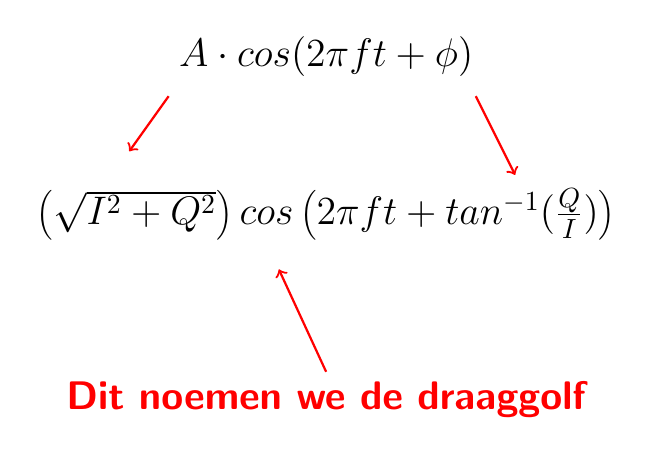
\begin{tikzpicture}[font=\Large\bfseries\sffamily]
   \draw (0,0) node[align=center]{$A\cdot cos(2\pi ft+ \phi)$}
   (0,-2) node[align=center]{$\left(\sqrt{I^2+Q^2}\right)cos\left(2\pi ft + tan^{-1}(\frac{Q}{I})\right)$};
   \draw[->,red,thick] (-2,-0.5) -- (-2.5,-1.2);
   \draw[->,red,thick] (1.9,-0.5) -- (2.4,-1.5);
   \draw[->,red,thick] (0,-4) node[red, below, align=center]{Dit noemen we de draaggolf} -- (-0.6,-2.7); 
\end{tikzpicture}
\end{document}